\documentclass[fleqn,10pt]{SelfArx} % Document font size and equations flushed left

\usepackage{float}
\usepackage{graphicx}
\usepackage{caption}
\usepackage[hyphens]{url}
\usepackage{hyperref}
\usepackage{xcolor}
\usepackage{amsmath}
\graphicspath{{../figures/}}
\setlength{\abovecaptionskip}{15pt plus 3pt minus 2pt}

\newcommand{\beginsupplement}{%
        \setcounter{table}{0}
        \renewcommand{\thetable}{S\arabic{table}}%
        \setcounter{figure}{0}
        \renewcommand{\thefigure}{S\arabic{figure}}%
     }

\definecolor{color1}{RGB}{0,0,90} % Color of the article title and sections
\definecolor{color2}{RGB}{200,200,200} % Color of the boxes behind the abstract and headings
\definecolor{color3}{RGB}{5,5,5} % Color of the boxes behind the abstract and headings

\JournalInfo{.} % Journal information ``Journal, Vol. XXI, No. 1, 1-5, 2015''
\Archive{ } % Additional notes (e.g. copyright, DOI, review/research article)

\PaperTitle{A meta-analysis of bioinformatics software benchmarks reveals that publication-bias unduly influences software accuracy} % Article title

\Authors{Paul P. Gardner\textsuperscript{1,2,3}*, James M. Paterson\textsuperscript{1,2}, Fatemeh Ashari-Ghomi\textsuperscript{1,2}, Sinan U. Umu\textsuperscript{1,2}, Stephanie McGimpsey\textsuperscript{4,5}, Aleksandra Pawlik\textsuperscript{6}} % Authors
\affiliation{\textsuperscript{1}\textit{School of Biological Sciences, University of Canterbury, Christchurch, New Zealand.}} % Author affiliation
\affiliation{\textsuperscript{2}\textit{Biomolecular Interaction Centre, University of Canterbury, Christchurch, New Zealand.}}
\affiliation{\textsuperscript{3}\textit{Bio-Protection Research Centre, University of Canterbury, Christchurch, New Zealand.}}
\affiliation{\textsuperscript{4}\textit{McConomy School of Dance, Derry, Ireland.}}
\affiliation{\textsuperscript{5}\textit{Research for Good, Limavady, Ireland.}}
\affiliation{\textsuperscript{6}\textit{New Zealand eScience Infrastructure, 49 Symonds St, Auckland, New Zealand.}}
\affiliation{*\textbf{Corresponding author}: paul.gardner@canterbury.ac.nz} % Corresponding author

\Keywords{} % Keywords - if you don't want any simply remove all the text between the curly brackets
\newcommand{\keywordname}{Keywords} % Defines the keywords heading name

%----------------------------------------------------------------------------------------
%	ABSTRACT
%----------------------------------------------------------------------------------------

%\Abstract{In the below we provide additional results for our investigation of computational biology benchmarks.}
\Abstract{
Computational biology has provided widely used and powerful software tools for testing and making inferences about biological data. In the face of increasing volumes of data, heuristic methods that trade software speed for mathematical completeness must be employed. 
We are interested in whether trade-offs between speed and accuracy are reasonable. Also, what factors are indicative of accurate software?

In this work we mine published benchmarks of computational biology software, we collect data on the relative accuracy and speed of different software and then test to see what factors influence accuracy e.g. speed, author reputation, journal impact or recency.

We found that author reputation, journal impact, the number of citations, software speed and age are not reliable predictors of software accuracy. This implies that useful bioinformatics software is not only the domain of famous researchers, and that any researchers are capable of producing good software. In addition, we found that there exists an excessive number of slow and inaccurate software tools across multiple sub-disciplines of bioinformatics. Meanwhile, there are very few tools of middling accuracy and speed. We hypothesise that a strong publication bias is unduly influencing the publication and development of bioinformatic software tools. In other words, at present software that is not highly ranked on speed and not highly ranked on accuracy is difficult to publish due to editorial and reviewer practices. This leaves an unfortunate gap in the literature upon which future software refinements could be constructed.
}

\begin{document}

\flushbottom % Makes all text pages the same height
\maketitle % Print the title and abstract box
%\tableofcontents % Print the contents section

\thispagestyle{empty} % Removes page numbering from the first page

%----------------------------------------------------------------------------------------
%	ARTICLE CONTENTS
%----------------------------------------------------------------------------------------

%\onecolumn
%\beginsupplement



%----------------------------------------------------------------------------------------
%	ARTICLE CONTENTS
%----------------------------------------------------------------------------------------

\section*{Background}
Computational biology software is widely used and has produced some of the most cited publications in the scientific corpus \cite{Perez-Iratxeta2007-lv,Van_Noorden2014-kc,Wren2016-xy}. This software includes implementations of methods for sequence alignment and homology inference \cite{Altschul1990-ht,Thompson1994-eu,Thompson1997-rl,Altschul1997-ga}, phylogenetic analysis \cite{Felsenstein1985-lj,Saitou1987-zl,Posada1998-qq,Ronquist2003-yh,Tamura2007-ei}, statistical analysis of survival patterns in biomedicine \cite{Kaplan1958-ju,Cox1972-nu}, biomolecular structure analysis \cite{Sheldrick1990-kc,Sheldrick2008-xy,Jones1991-ik,Laskowski1993-vi,Otwinowski1997-xj}, visualization and data collection \cite{Kraulis1991-lt,Berman2000-to}. However, the popularity of a software tool does not necessarily imply that it is either accurate or computationally efficient, instead usability, ease of installation, operating system and other factors may play a greater role.

Progress in the biological sciences is increasingly limited by the ability to analyse increasing volumes of data, therefore the dependence of biologists on software is also increasing \cite{Marx2013-zi}. There is an increasing use of technological solutions for automating biological data generation (e.g. next-generation sequencing, mass-spectroscopy, cell-tracking and species tracking), therefore the biological sciences have become increasingly dependent upon computational software for processing large quantities of data \cite{Marx2013-zi}. As a consequence, the computational efficiency of data processing and analysis software is of great importance to decrease the energy and time costs of research \cite{Gombiner2011-md}. Furthermore, even small error rates can have a major impact on the number of false inferences as datasets become larger \cite{Storey2003-cv}.

The gold-standard for determining accuracy is for independent researchers to conduct benchmarks, which can serve a useful role in reducing the over-optimistic reporting of software accuracy \cite{Boulesteix2010-te,Jelizarow2010-zf} and the self-assessment trap \cite{Norel2011-cq}. Benchmark studies typically use a number of positive and negative control datasets, predictions can then be partitioned into true or false groups and a variety of metrics can be used to evaluate the performance of different predictions \cite{Egan1975-nd,Hall2012-kg}. Some benchmarks now use live, or frequently updated, results to indicate the latest developments in software performance \cite{Bujnicki2001-xr,Puton2014-hy,Barton_undated-er}. The aim of these benchmarks is to independently identify tools that make acceptable compromises in terms of scoring schemes and the resulting potential for false predictions, true predictions and speed, and are therefore suited for wide adoption by the community.

For common computational biology tasks, a proliferation of software-based solutions often exists \cite{Felsenstein1995-ic,Altschul2013-bv,Henry2014-ut,Wikipedia_contributors2015-vj,Wikipedia_contributors2015-hr}. While this may generally be a good problem to have, and points to a diversity of options from which practical solutions can be selected, many possible options creates a dilemma for users. In the absence of any recent gold-standard benchmarks, how should scientific software be selected? In the following work, we presume that ``biological accuracy'' is the most desirable feature of software. Biological accuracy is the degree to which predictions or measurements reflect the truths of biological systems, this is usually determined by comparing results of software to the results of established reference data. These are commonly expert-derived curated datasets. In some fields biological accuracy is very difficult to ascertain, for example, in phylogenetics it is nearly impossible to know the ancestral relationships between organisms. In situations like this, researchers can use a mix of simulated or high-confidence datasets.

A number of possible predictors of software quality are used by the community of computational biology software users. Some accessible, quantifiable and frequently used proxies for identifying high quality software include: \textbf{1. Recency:} recently published software tools may have built upon the results of past work or be an update to an existing software. Therefore, these could be more accurate and faster. \textbf{2. Wide adoption:} a software tool may be widely used because it is fast and accurate, or because it is well-supported and user-friendly. In fact, “large user base”, “word-of-mouth”, “wide-adoption”, "personal recommendation," and "recommendation from a close colleague," are frequent responses to surveys of “how do scientists select software?” \cite{Hannay2009-cf,Joppa2013-vj,Loman2015-bw}. \textbf{3. Journal impact:} high profile journals are run by editors and reviewers who carefully select and curate the best manuscripts. Therefore, high impact journals may be more likely to select manuscripts describing good software \cite{Garfield1955-wf}. \textbf{4. Author/Group reputation:} the key to any project is the skills of the people involved, including maintaining a high collective intelligence \cite{Joppa2013-vj,Woolley2010-ld,Cheruvelil2014-xn}. As a consequence, an argument could be made that well respected and high-profile authors will produce better software \cite{Hirsch2005-mt,Bornmann2008-il}. \textbf{5. Speed:} software is frequently said to trade accuracy for speed. For example, heuristic software such as the popular homology search tool, BLAST, compromise the mathematical guarantee of optimal solutions for more speed \cite{Altschul1990-ht,Altschul1997-ga}. Some researchers may naively interpret this fact as slower software is likely to be more accurate. But speed may also be influenced by the programming language \cite{Fourment2008-vl}, and/or level of hardware optimisation \cite{Farrar2007-ky,Dematte2010-ph}; In general the implementation is likely to have more of an impact (e.g. brute-force approaches versus rapid and sensitive pre-filtering \cite{Schaeffer1989-mu,Papadimitriou_undated-bo}).

Other factors that influence whether a software tool is selected include: whether the documentation is good, user-friendly, word-of-mouth and ``used in a similar analysis'' \cite{Loman2015-bw}. This sort of information is not as readily quantifiable as the above measures. However, citation metrics may be a useful proxy. The word-of-mouth factor may also explain the reason why some software continues to be used, in spite of poor relative performance \cite{Wadi2016-dj}.

In the following study, we explore factors that may be indicative of software accuracy. This, in our opinion, should be one of the prime reasons for selecting a software tool. We have mined the large and freely accessible PubMed database \cite{Sayers2010-vm} for benchmarks of computational biology software, and manually extracted accuracy and speed rankings for \textbf{{\color{black}243}} software packages. For each software tool, we have collected measures that may be predictive of accuracy, and may be subjectively employed by the researcher community as a proxy for software quality. These include relative speed, relative age, the productivity and impact of the corresponding authors, journal impact and the number of citations. 

\section*{Results}
We have collected relative accuracy and speed ranks for \textbf{{\color{black}243}} distinct software tools. This software has been developed for solving a broad cross-section computational biology tasks. These include software for homology search \cite{Freyhult2007-et}, genome sequence analysis (e.g. read mapping or sequence assembly) \cite{Junemann2014-mb,Tran2014-pe,Zhang2011-nd,Abbas2014-gu,Bao2011-lv,Caboche2014-lj,Kleftogiannis2013-wi,Hatem2013-cs,Schbath2012-ob,Ruffalo2011-rl,Yang2013-aj,Holtgrewe2011-fd,Rackham2015-ag,Huang2015-wu}, multiple sequence alignment \cite{Thompson2011-rf,Nuin2006-nk,Pais2014-sr,Pervez2014-zp,Liu2010-rp}, cell tracking \cite{Maska2014-ak}, transcriptome analysis \cite{Li2012-wr,Lu2013-fs,Liu2014-kz,Kumar2016-xz}, RNA interaction prediction \cite{Pain2015-gr}, protein interactions \cite{Tikk2010-qd}, protein structure prediction \cite{Kolodny2005-ry,Wallner2005-qi}, epistasis \cite{Shang2011-vy},  metagenomic analysis \cite{Lindgreen2016-tt,Bazinet2012-wf}, repetitive sequence prediction \cite{Saha2008-kd}, proteomics \cite{Lange2008-pt,Yang2009-oc} and phylogenetics \cite{Liu2011-pz,Yang2011-dv,Oscamou2008-md,Bayzid2013-hc,Liu2009-lx}. Each software tool was benchmarked in at least one of \textbf{{\color{black}43}} publications that satisfy the Boulesteix criteria \cite{Boulesteix2013-vb}. In brief, the Boulesteix criteria are: 1. the main focus of the article is a benchmark. 2. the authors are reasonably neutral. 3. the test data and evaluation criteria are sensible.

For each of the publications describing these methods, we have (when possible) identified the 2014 journal impact factor (JIF), published by Thomson Reuters \cite{Garfield2006-lv} and the H5-index published by \href{https://scholar.google.co.nz/citations?view_op=top_venues&hl=en}{Google Scholar Metrics}. We have collected the H-indices and M-indices \cite{Hirsch2005-mt} for the corresponding authors for each method, and the number of times the publication(s) associated with a method has been cited using Google Scholar (data collected over a 1 month period in early 2016).

We have computed the Spearman’s correlation coefficient for each pairwise combination of the mean normalised accuracy and speed ranks, the year published, mean relative age (compared to software in the same benchmarks), journal IF and H5 metrics, the total number of citations, the relative number of citations (compared to software in the same benchmarks) and the maximum H and M indices for the corresponding authors. The results are presented in Figure~\ref{fig:allfactors}A. We found significant associations between most of the citation-based metrics (journal H5, JIF, citations, relative citations, H-index and M-index). There is also a strong association between the year of publication, the relative age and many of the citation-based metrics.

\begin{figure*}[h]
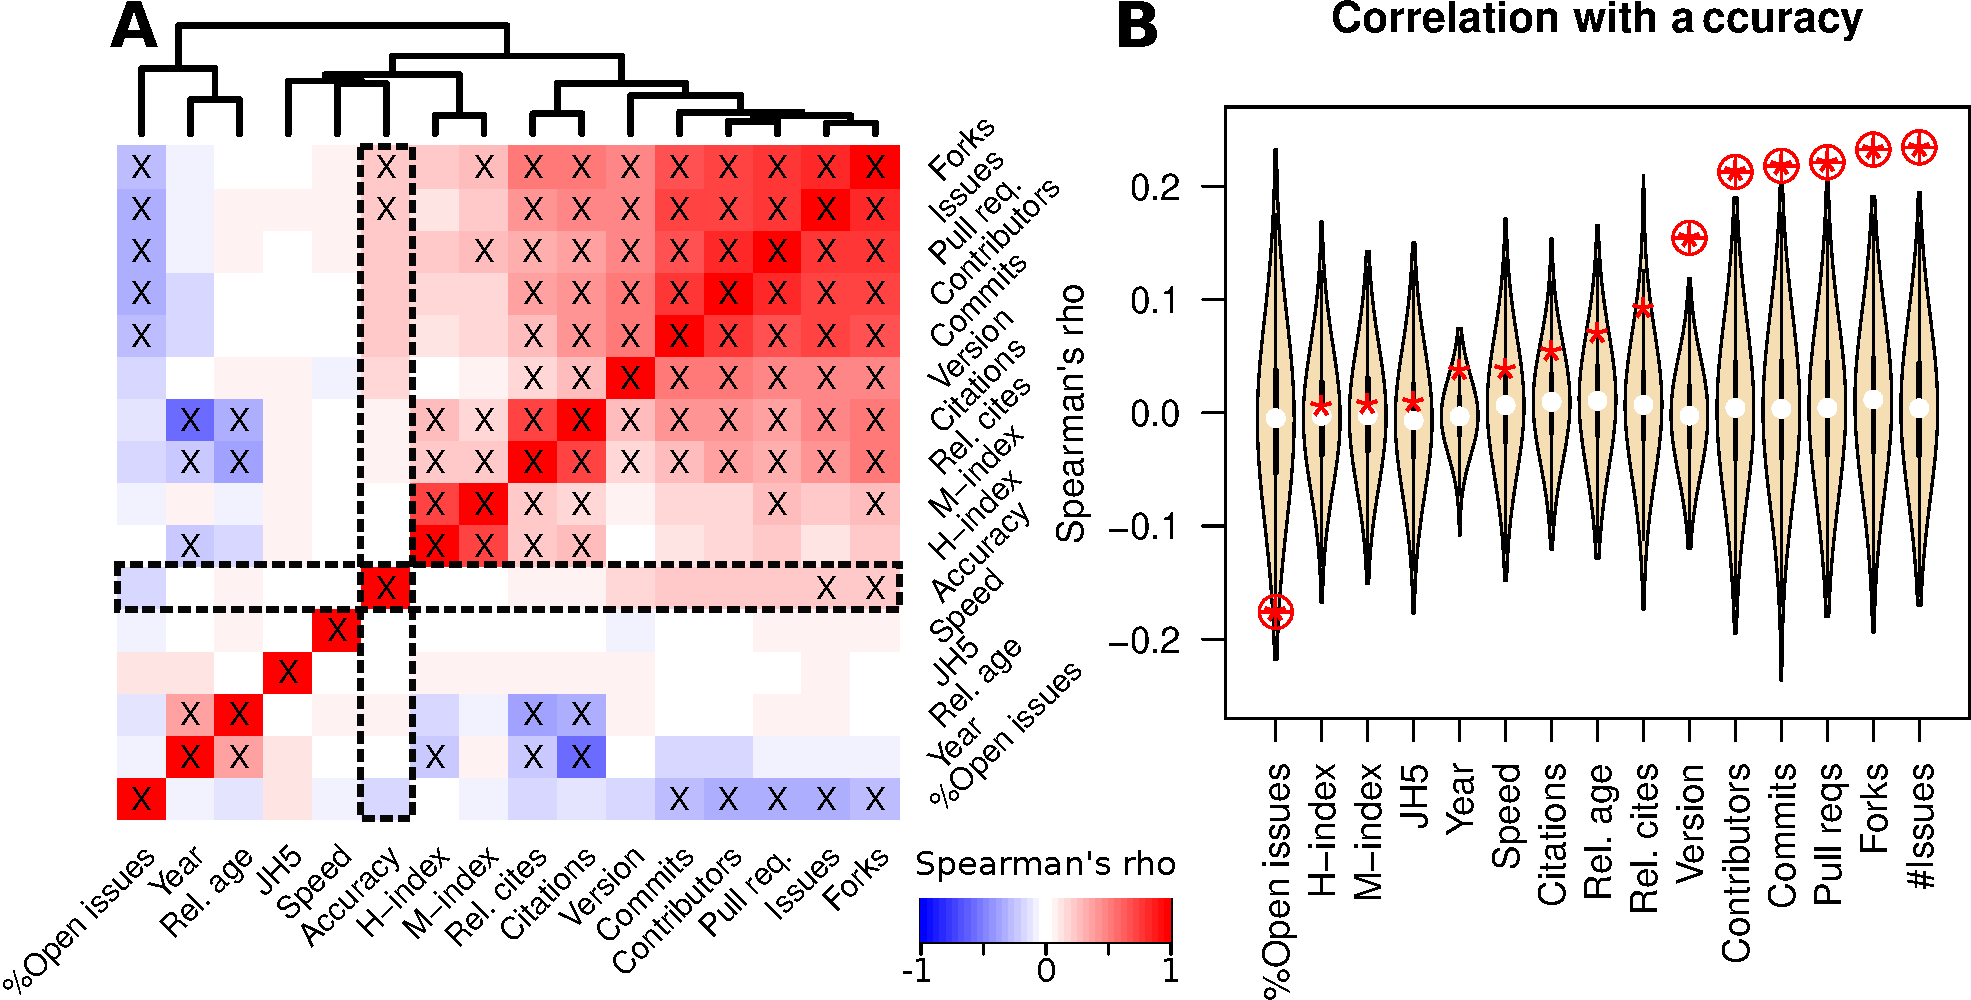
\includegraphics[width=\textwidth]{figure1.pdf}
\caption{\textbf{A.} A heatmap indicating the relationships between proposed predictors of software quality. Spearman’s rho is used to infer correlations between metrics such as the H and M indices of corresponding authors, number of citations, journal impact factors and H5 indices, the year and relative age of software and the mean relative rankings of software speed and accuracy. Red colours indicate a high positive correlation, blue colours indicate a high negative correlation. Correlations with a P-value less than 0.05 are indicated with a ‘X’. The dashed rectangular area is illustrated in more detail in \textbf{B}, the bold square is shown in more detail in \textbf{Figure 2}.The dendrogram was computed using the default ‘heatmap.2 function in R, which computes a Euclidean distance matrix and a complete-linkage hierarchical clustering. \textbf{B.} A barplot illustrating the correlation as measured by Spearman’s rho between and normalised accuracy ranks and potential factors that may be predictive of accuracy. In order to give an appreciation of the difference between the observed effect-sizes and significant effect sizes, we generated 10,000 permuted accuracy ranks for each benchmark and recorded Spearman’s rho for the significant correlations (P<0.05). These values are marked with “x”s in the barplot.}
\label{fig:allfactors}
\end{figure*}


We found that author reputation metrics, journal impacts and the age of methods were \textbf{not} significantly correlated with either method accuracy or speed (see Figure~\ref{fig:allfactors}). The strongest association was between accuracy and journal impact factor (Spearman’s rho = 0.1, P-value = 0.16). A linear model of these parameters and accuracy also failed to identify a correlation between these (accuracy: R2 = -0.03, P-value = 0.94; speed: R2 = 0.04, P-value = 0.66). To further validate this result, we compute a correlation between speed and accuracy for each benchmark and used weighted sum Z-tests \cite{Zaykin2011-tj}. This also failed to identify a significant relationship (sum Z=-0.1, P-value=0.5).

In order to gain a deeper understanding of the distribution of available bioinformatic software tools on a speed versus accuracy landscape, we ran a Monte Carlo permutation test. The ranks extracted from each benchmark were randomly permuted, generating 10,000 randomized speed and accuracy ranks. In the cells of a $10\times10$ grid spanning the normalised speed and accuracy ranks we computed a Z-score for the observed number of methods in a cell, compared to the expected distributions generated by the randomized ranks. The results of which are shown in Figure~\ref{fig:speedaccuracy}. We identified 21 bins where there was a significant excess or dearth of methods. For example, there was an excess of “slow and inaccurate” software (Z=1.6, P-value=0.05) and “slow and accurate” software (Z=1.9, P-value=0.03). We find that the amount of software classed as “fast and accurate” and “fast and inaccurate” are at approximately the expected proportions based upon the permutation test. The number of significant results is in excess and not due to multiple testing, as the probability of finding 21 of 100 tests significant by chance is low (P-value = $2\times 10^{-8}$, exact binomial test) \cite{Moran2003-ve}.


\begin{figure*}
%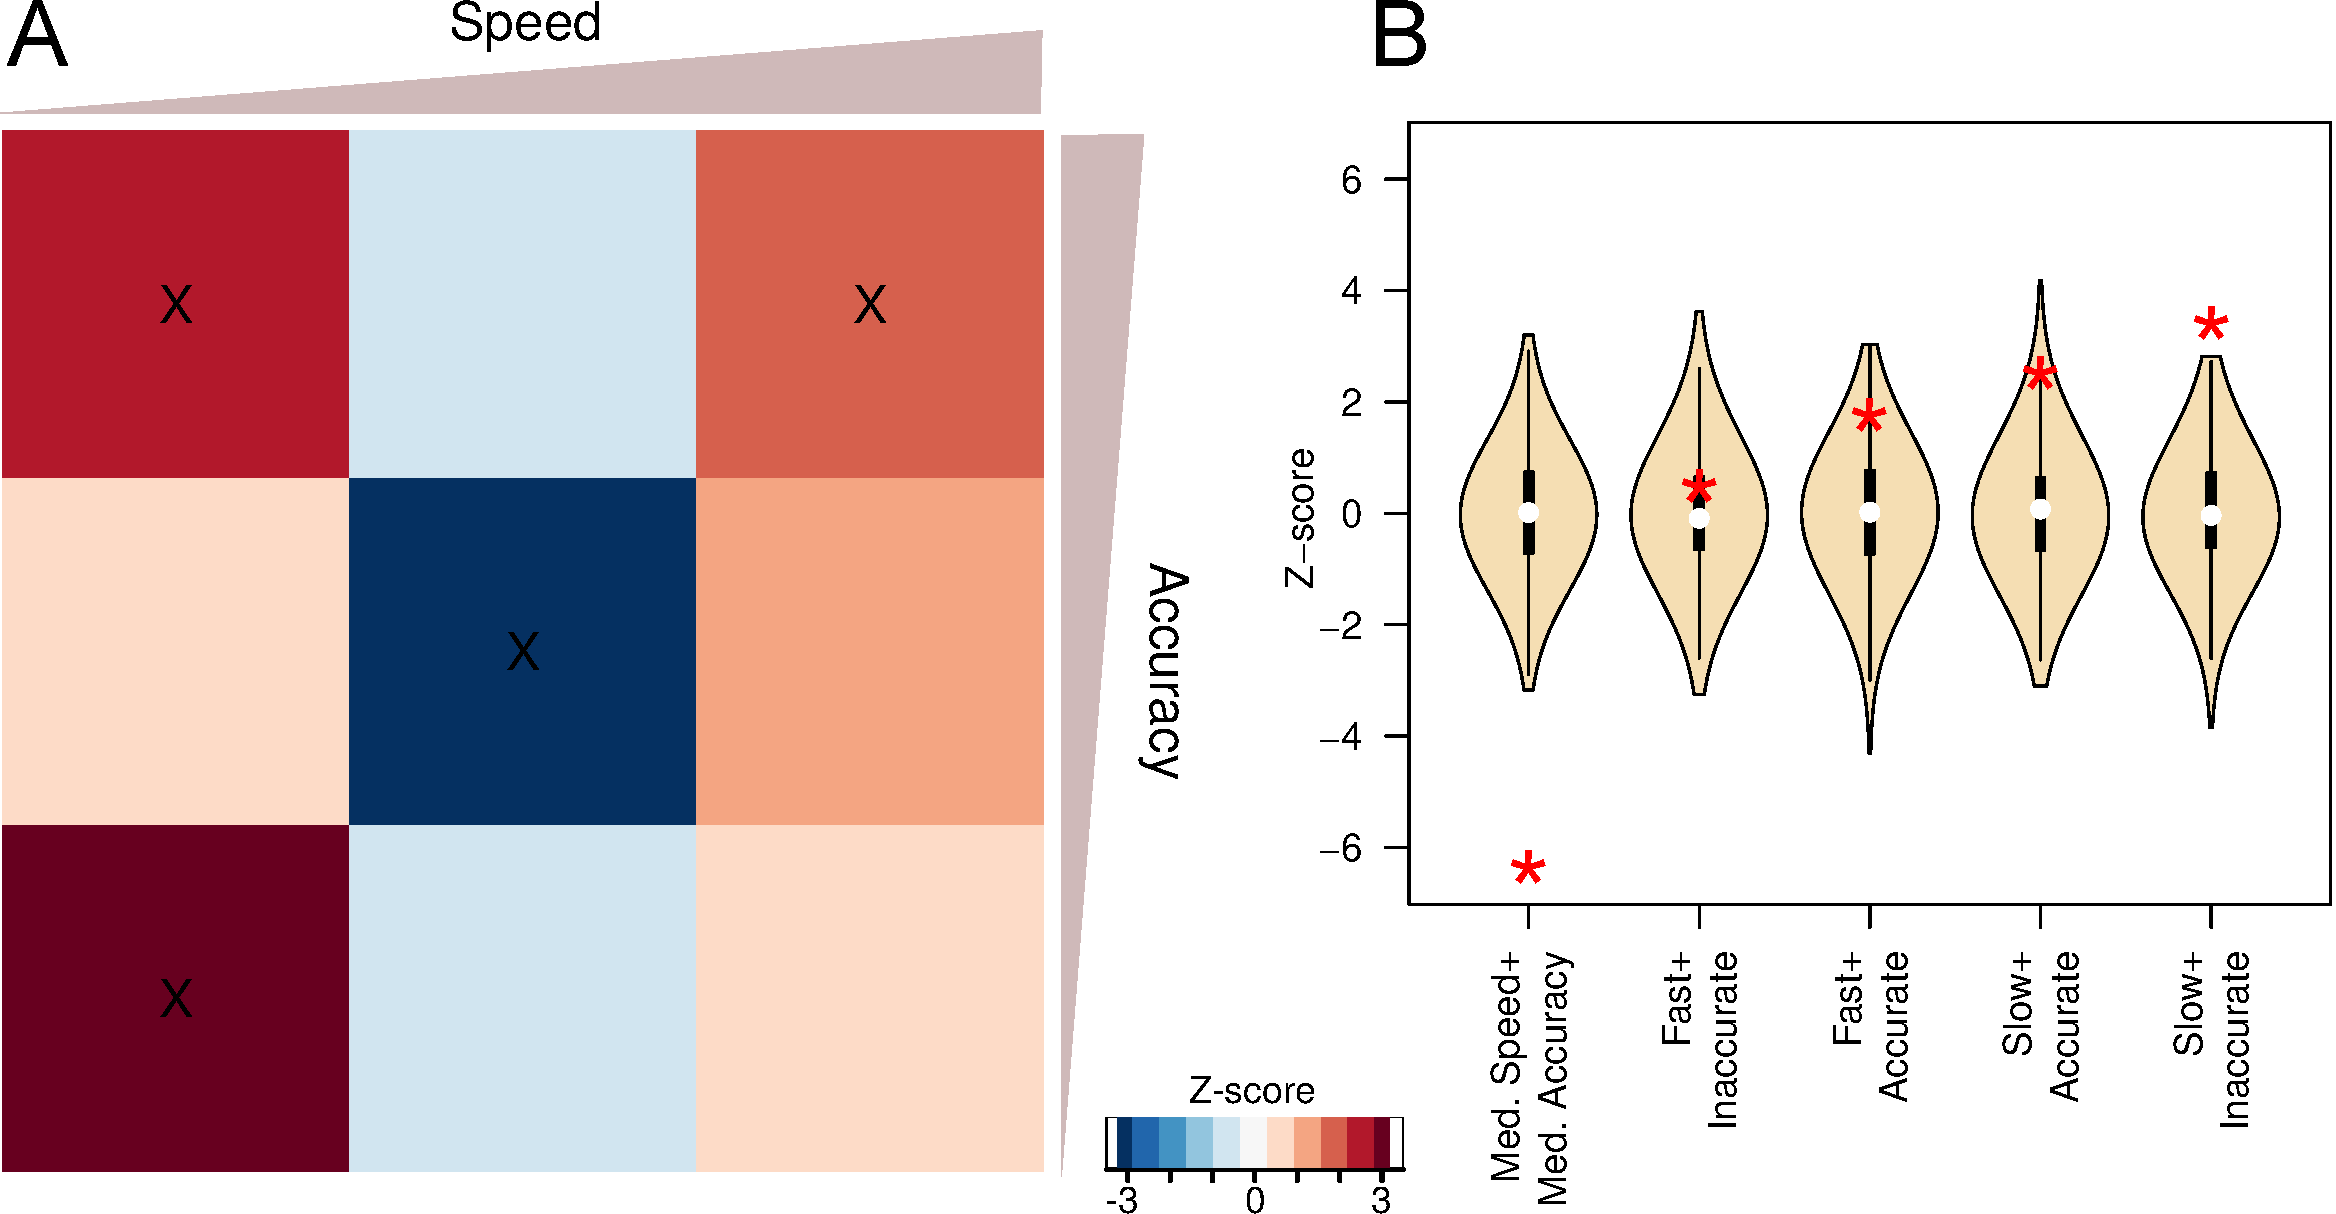
\includegraphics[scale=0.55]{figure2.pdf}
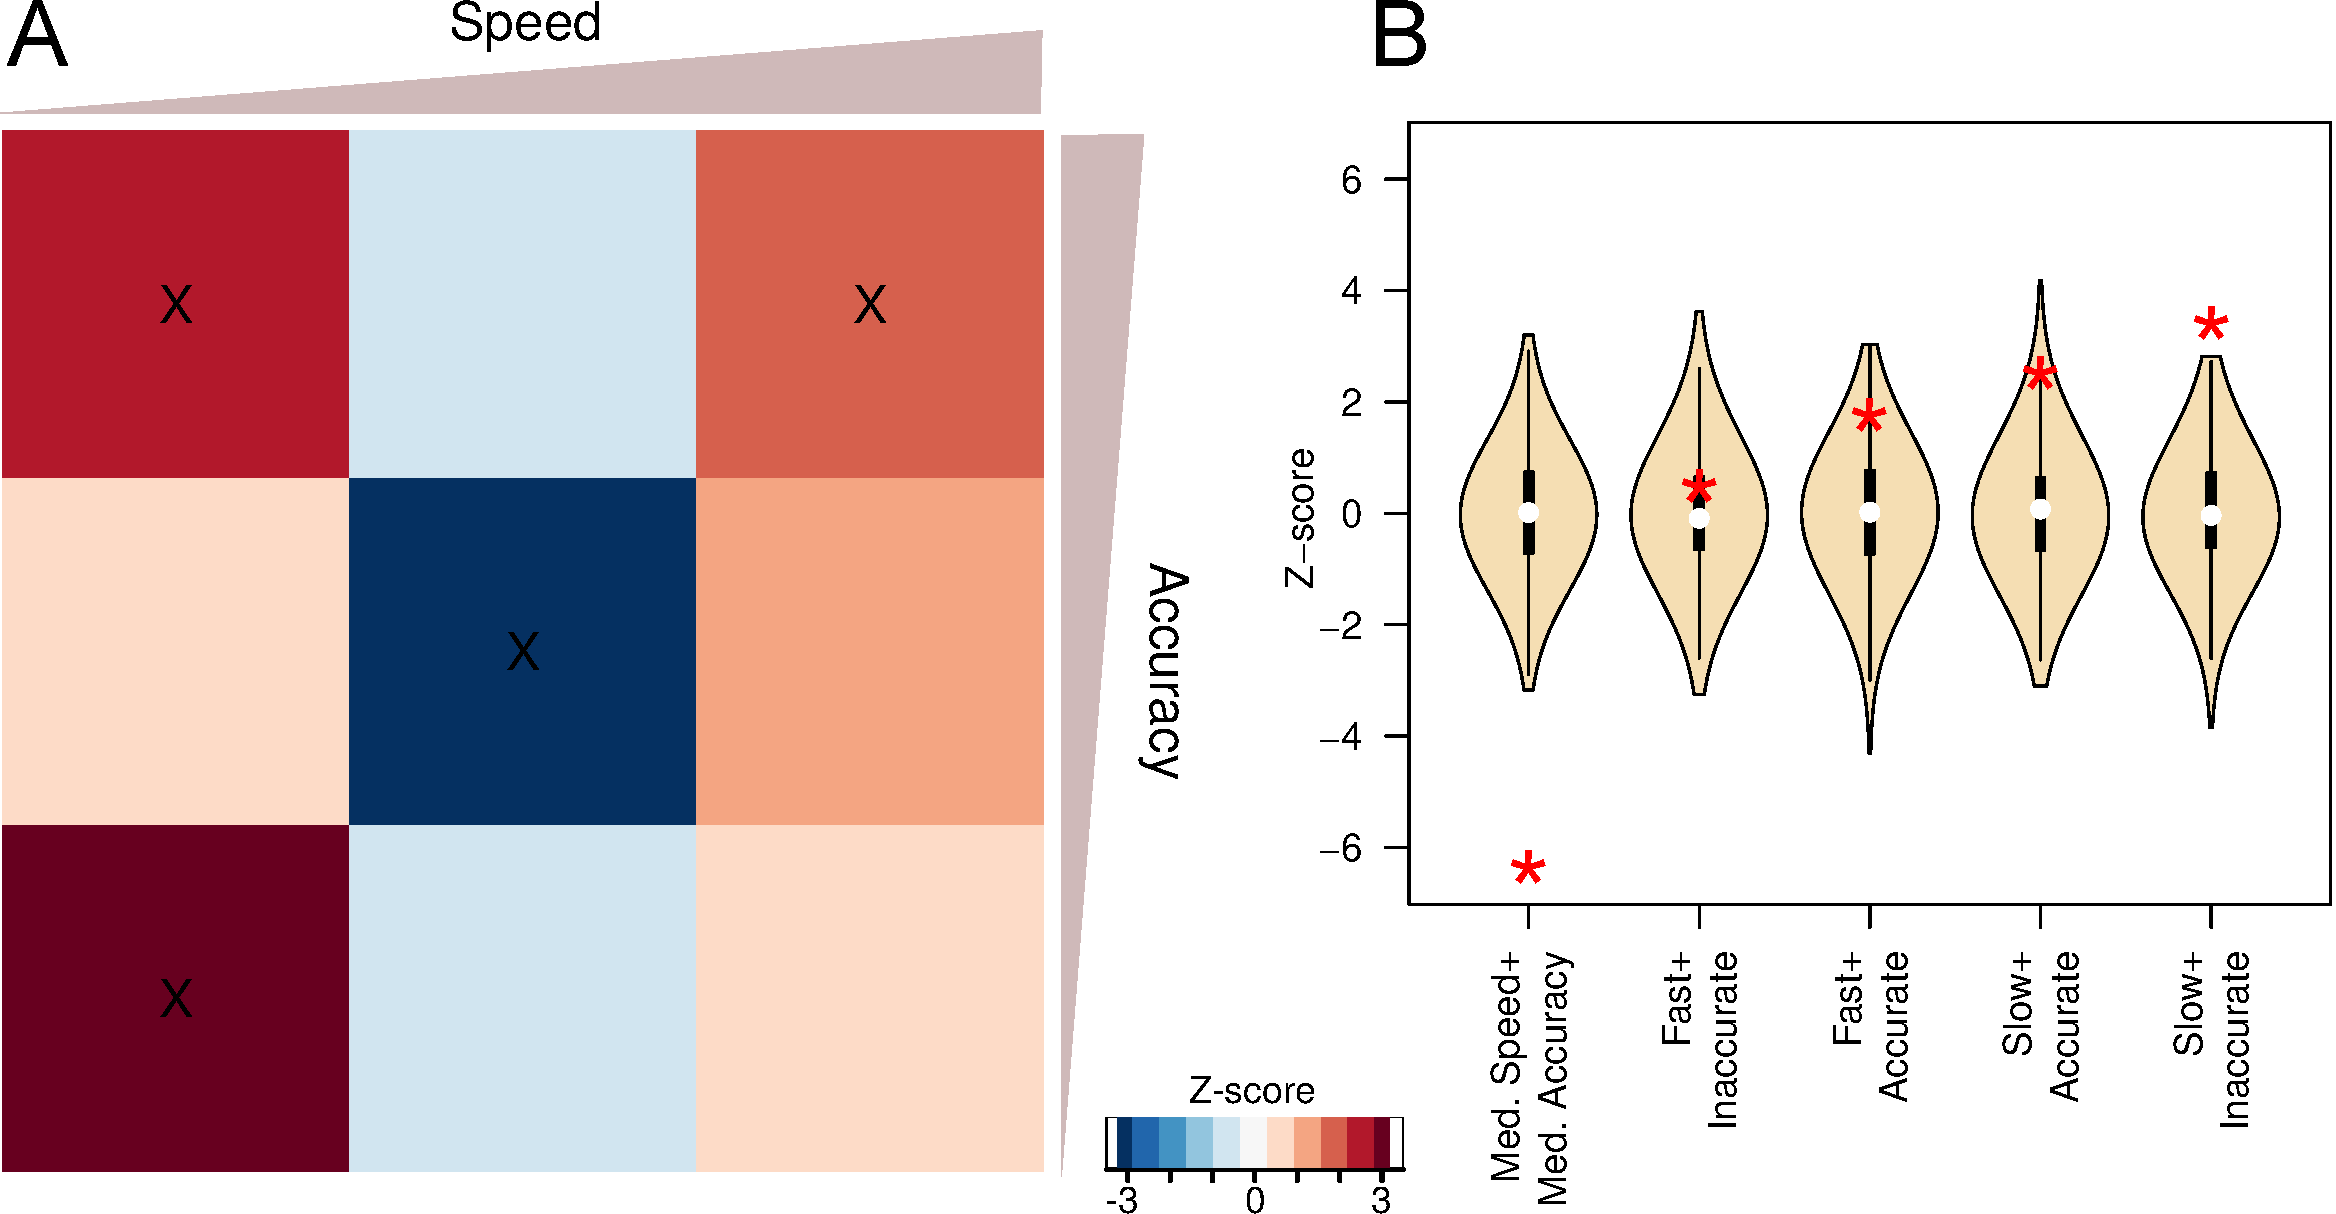
\includegraphics[width=\textwidth]{figure2.pdf}
\caption{A heatmap indicating the relative paucity or abundance of software in the range of possible accuracy and speed rankings. Red colours indicate an abundance of software tools in an accuracy and speed category, while blue colours indicate scarcity of software in an accuracy and speed category. The abundance is quantified using a Z-score computation for each bin, this is derived from 10,000 random permutations of the speed and accuracy ranks from each benchmark. Mean normalised ranks of accuracy and speed have been binned into 100 classes (a $10\times10$ grid) that range from comparatively slow/inaccurate to comparatively fast/accurate. Z-scores with a P-value less than 0.05 are indicated with a ‘X’.}
\label{fig:speedaccuracy}
\end{figure*}

There is a large reduction in the number of software tools that are classed as intermediate in terms of both speed and accuracy based upon our permutation test (Figure~\ref{fig:speedaccuracy}). The cells corresponding to the four central underrepresented deciles are highlighted (Z = -1.7, -2.1, -2.1 and -2.4, P-values = 0.04, 0.02, 0.02 and 0.008, respectively, reading from top to bottom, left to right). We also tested the relative age of the software tools in significantly over- or under-represented regions of the speed vs accuracy plot. We found that the “slow and inaccurate” methods were generally published earlier than other methods (W = 31, P=0.007, one-tailed Wilcoxon test) (Figure S8).

\section*{Discussion}

We have gathered data on the relative speed and accuracies of \textbf{{\color{black}243}} bioinformatic methods from \textbf{{\color{black}43}} benchmarks that were published between 2005 and 2016. We show that there is an under-representation of software that has both intermediate levels of accuracy and speed. There may be a number of factors that drive this phenomena. One likely explanation is that bioinformatic software tools suffer from a form of publication bias \cite{Boulesteix2015-am}. Our community of developers, reviewers and editors may be unwilling to publish software that is neither the fastest nor the most accurate (we have anecdotal evidence to support this, N=1). If correct, this is unfortunate. Some problems that lack fast and accurate solutions force researchers to make unnecessary compromises in terms of accuracy and time. If our hypothesis that this underrepresentation is due to publication bias is valid then why is there an enrichment of slow and inaccurate software (P-value=0.05, empirical distributions from permutation tests)? How could these methods be published? We have found that slow and inaccurate software is generally published earlier than alternative methods (P=0.007, one-tailed Wilcoxon test), therefore comparisons were not required to publish these tools and the accuracies may have been over-optimistically reported \cite{Boulesteix2015-nc}.

We found that no commonly used proxy for study quality is correlated with software accuracy. Neither, author reputation, number of citations, journal impact, relative age or speed appear to be associated with accurate software. Linear mixed models of these values also fail to identify predictors of software accuracy, as do methods for combining P-values. A great deal of criticism has been leveled specifically at journal impact factors \cite{Editors2006-ue,Rossner2007-yk,Lariviere2010-kx}. Our finding show that this measure is not reflective of software quality. But neither is the H5 index which is thought to be a more robust measures of journal impact \cite{Harzing2008-wb}. The poor relationship between accuracy and both author reputation and the number of citations is particularly troubling. Both are related to “word of mouth” and “previously used in a similar analysis” which a recent survey of researchers suggested is a major influence on the selection of software tools \cite{Loman2015-bw}. This implies that the recorded high citation rates for bioinformatic software  \cite{Perez-Iratxeta2007-lv,Van_Noorden2014-kc,Wren2016-xy} is more a reflection of user-friendliness and the Matthew Effect \cite{Lariviere2010-kx,Merton1968-cb}. The Matthew Effect is a biblical reference that can be paraphrased as “the rich get richer and the poor get poorer”. In this context, highly cited software is more likely to be used and cited again, irrespective of relative performance. 

The lack of any relationship between software speed and accuracy is surprising. 
The slower software tools are found to be overrepresented at both high and low levels of accuracy (Figure~\ref{fig:speedaccuracy}). Likewise accurate software was found in both high and low speed ranges. A simple gedankenexperiment may be sufficient to prove that slow software is less thoroughly tested than fast software. This is because typical software development is an iterative process, where methods are refined by successive rounds of coding, testing and evaluation \cite{Wilson2006-ih}. We can assume that similar time-spans are spent on most projects, for example, the span of a MSc or PhD degree.  As a consequence slow software undergoes fewer development cycles than fast methods, and is therefore tested less, often resulting in less accurate and slower software. The fact that fast and inaccurate software is relatively rare does support this argument. The lack of any further apparent relationship between speed and accuracy implies there are stronger influences on accuracy rankings than speed alone.

\section*{Conclusions}
Scientific progress is a grinding process made by testing hypotheses using appropriate positive and negative controls, in combination with independent experiments and replication \cite{Ioannidis2005-xh,Moonesinghe2007-kk}. We think that software and analysis tools should be no exception to these principles. The continual increases in the complexity of software tools creates an increased likelihood that software bugs are introduced \cite{Darriba2015-sz}. Scientific software should therefore be thoroughly tested by developers, however, the results of developer and author-derived tests should be treated with caution due to a range of potential conscious and unconscious biases \cite{Norel2011-cq}. Our study shows that no commonly-used impact-based metrics are related to software accuracy, therefore the only reasonable way to select software tools is through software benchmarks.

We have shown that slow and inaccurate software is typically published early in the development of a field (see Figure S8). Subsequent software tools may be high accuracy or high speed. However, as further software tools become available, those that do not rank highly in terms of accuracy or speed are under-represented in the literature. Our conjecture is that this is due to a publication bias in computational biology software literature, with publishers, editors and reviewers implicitly requiring software to be notable in at least one of these regards in order to be published. This hole in the literature leaves an unfortunate gap upon which further software refinements cannot be made. 

The software that could be used in building research workflows can make use of software tools that are of medium accuracy and speed. These may prove to be useful rapid pre-filters for more accurate, yet computationally-demanding approaches. These could also be used when datasets are too large to be processed by more accurate software tools, i.e. when accurate tools are slow or memory hungry \cite{Lowe1997-hq,Weinberg2006-tm}. These tools may also serve as an indication that some approaches may not be worth pursuing further.

We propose that the full spectrum of software tool accuracies and speeds serve a useful purpose to the research community. Like negative results, if honestly reported, illustrate to the research community that certain approaches are not practical research avenues \cite{Ioannidis2005-xh,Workman1999-au,Rivas2000-fb}. The classes of tools that we find in the under-represented accuracy and speed region include some of the most used tools in bioinformatics, such as the homology search tools NCBI-BLAST \cite{Altschul1990-ht,Altschul1997-ga} and HMMER \cite{Eddy:2009} and genome assembly and mapping tools such as AbySS \cite{Simpson:2009}, MAQ \cite{Li:2008} and Newbler \cite{Margulies:2005}. The current practises of publishers, editors, reviewers and authors of software tools therefore deprive our community of tools for building effective and productive workflows.

A potential avenue for further exploration is to compare the starting point for software development projects as certain approaches may produce more rapid gains than others. For example, starting with biologically plausible and fast methods will theoretically allow more rapid gains in accuracy through iterative method refinement than starting with slow and mathematically complete approaches. At the very least these may be used as rapid data filters for reducing the size and complexity of problems, prior to employing more rigorous methods. 


We have shown that accurate software is not necessarily the most recently released method or the product of high profile lab groups or selected by high impact journals. Software that is widely used or is either slow or fast is also not necessarily the most accurate. Therefore, accurate software may be the product of features we have not been able to capture. Possibly, hard work, good ideas and sound method testing, as well as technical ability, experience and education levels in software development \cite{Wilson2006-ih}. 


Finally, we think that the field of computational biology could benefit from embracing an increased number of independent software comparison studies \cite{Boulesteix2013-vb}, in parallel with the popular challenge-based benchmarks such as CASP, Assemblathon, Alignathon, DREAM and RGASP \cite{Boutros2014-zm}. We are hopeful that this, along with the relaxation of the publication bias we have described, will reduce the over-optimistic and misleading reporting of method accuracy \cite{Boulesteix2010-te,Jelizarow2010-zf,Norel2011-cq}. 

\section*{Methods}
In order to evaluate predictors of computational biology software accuracy, we mined the published literature, extracted data from articles, connected these with bibliometric databases, and tested for correlates with accuracy. We outline these steps in further detail below. 

\textbf{Criteria for inclusion:} We are interested in using computational biology benchmarks that satisfy Anne-Laure Boulesteix’s (ALB) three criteria for a “neutral comparison study” \cite{Boulesteix2013-vb}. Firstly, the main focus of the article is the comparison and \textbf{not} the introduction of a new method. Secondly, the authors should be reasonably neutral, which means that the authors should not generally have been involved in the development of the methods included in the benchmark. Thirdly, the test data and evaluation criteria should be sensible. This means that the test data should be independent of data that methods have been trained upon, and that the evaluation measures appropriately quantify correct and incorrect predictions.

Literature mining: We identified an initial list of 10 benchmark articles that satisfy the ALB-criteria. These were identified based upon previous knowledge of published articles and were supplemented with several literature searches (e.g. ‘“benchmark” AND “cputime”’ was used to query both GoogleScholar and Pubmed \cite{Sayers2010-vm,McEntyre2001-fl}). We used these articles to seed a machine-learning approach for identifying further candidate articles and to identify new search terms to include.

For our machine-learning-based literature screening, we computed a score ($s(a)$) for each article that tells us the likelihood that it is a benchmark. In brief, our approaches uses 3 stages:
\begin{enumerate}
\item Remove high frequency words from the title and abstract of candidate articles (e.g. ‘the’, ‘and’, ‘of’, ‘to’, ‘a’, …) 
\item Compute a log-odds score for the remaining words 
\item Use a sum of log-odds scores to give a total score for candidate articles
\end{enumerate}
For stage 1, we identified a list of high frequency (e.g. f(word) $>$ 1/10,000) words by pooling the content of two control texts \cite{Carroll1865-hk,Tolkien1937-ke}. 

For stage 2, in order to compute a log-odds score for bioinformatic words, we computed the frequency of words that were not removed by our high frequency filter in two different groups of articles: bioinformatics-background and bioinformatics-benchmark articles. The text from bioinformatics-background articles were drawn from the bioinformatics literature, but these were not necessarily associated with benchmark studies. For background text we used Pubmed (\cite{Sayers2010-vm,McEntyre2001-fl} to select 8,908 articles that contained the word “bioinformatics” in the title or abstract and were published between 2013 and 2015. We computed frequencies for each word by combining text from titles and abstracts for the background and training articles. A log-odds score is computed for each word using the following formula: $lo(w)=\log_2\frac{•f_{tr}(word)+\delta}{f_{bg}(word)+\delta}$, where  is a prior probability ($\delta = 10^{-5}$, by default), $f_{bg}(word)$ and $f_{tr}(word)$ are the frequencies of a $word$ in the background and training datasets respectively. Word frequencies are computed by counting the number of times a word appears in the pool of titles and abstracts, the counts are normalised by the total number of words in each set. 

Thirdly, we also collected a group of candidate benchmark articles by mining Pubmed for articles that are likely to be benchmarks of bioinformatic software, these may match the terms: “((bioinformatics) AND (algorithms OR programs OR software)) AND (accuracy OR assessment OR benchmark OR comparison OR performance) AND (speed OR time)”. Further terms used in this search were progressively added as relevant enriched terms were identified in later iterations. The final query is given in \textbf{supplementary materials}.

A score is computed for each candidate article by summing the log-odds scores for the words in title and abstract, i.e. $s(a)=\sum_i^Nlo(w_i)$. The high scoring candidate articles are then manually evaluated against the ALB-criteria. Accuracy and speed ranks are extracted from the articles that meet the criteria, and these are also added to the set of training articles. The evaluated candidate articles that do not meet the ALB-criteria are incorporated into the set of background articles. This process is iterated a number of times and has resulted in the identification of \textbf{{\color{black}43}} benchmark articles, that contain \textbf{{\color{black}102}} different benchmarks, together these rank \textbf{{\color{black}243}} distinct software packages.

There is a potential for bias to have been introduced into this dataset. Some possible forms of bias include converging on a niche group of benchmark studies due to the literature mining technique that we have used. A further possibility is that benchmark studies themselves are biased, either including very high performing or very low performing software tools. To address each of these concerns we have attempted to be as comprehensive as possible in terms of benchmark inclusion, as well as include comprehensive benchmarks. By which we mean studies that include all available software tools that address a biological problem. 

\textbf{Data extraction and processing:} for each article that met the ALB-criteria and contained data on both the accuracy and speed from their tests we extracted ranks for each method. Many articles contained multiple benchmarks, in these cases we selected a range of these, the provenance of which is stored with the accuracy metric and raw speed and accuracy rank data for each method. In line with rank-based statistics, the cases where methods were tied are resolved by using a midpoint rank (e.g. if method 3 and 4 are tied, the rank 3.5 is used) \cite{Mann1947-re}. Each rank extraction was independently verified by at least one other co-author to ensure both the provenance of the data could be established and that the ranks were correct. The ranks for each benchmark were then normalised to lie between 0 and 1 using the formula $\frac{r-1}{n-1}$ where ‘r’ is a method’s rank and ‘n’ is the number of methods in the benchmark. For methods that were benchmarked multiple times with multiple metrics (e.g. BWA is evaluated in 6 different articles \cite{Bao2011-lv,Caboche2014-lj,Hatem2013-cs,Schbath2012-ob,Ruffalo2011-rl,Holtgrewe2011-fd}) a mean normalised rank is used to summarise the performance.
 
For each method we identified the corresponding publications in GoogleScholar, the total number of citations was recorded, the corresponding authors were also identified and if these had public GoogleScholar profiles we extracted their H-index and calculated a M-index ($\frac{H-index}{y}$) where ‘$y$’ is the number of years since their first publication. For the journals that each method is published in we extracted the “journal impact factor” (JIF) and the H5-index from Thompson-Reuters and GoogleScholar Metrics databases respectively. The year of publication was also recorded for each method. A “relative age” and “relative citations” was also computed for each method. For each benchmark, software was ranked by year of first publication (or number of citations), ranks were assigned and then normalised as described above. Methods ranked in multiple evaluations were then assigned a mean value for “relative age” and “relative citations”. 

\textbf{Statistical analysis:} For each method we have up to 10 statistics (1. corresponding author’s H-index, 2. corresponding author’s M-index, 3. journal H5 index, 4. journal impact factor, 5. normalised accuracy rank, 6. normalised speed rank, 7. number of citations, 8. relative age, 9. relative number of citations, 10. year first published). These have been evaluated in a pairwise fashion to produce Figure~\ref{fig:allfactors} A\&B, the R code for these is given in the supplement. 

The linear models that we used to test for relationships between speed, accuracy and the above measures are:

\begin{equation*}
\begin{split}
accuracy=& c_0+c_1\times speed+c_2\times JIF+c_3\times H5+\\
& c_4\times citations+c_5\times Hindex+\\
& c_6\times Mindex+c_7\times relativeAge+\\
& c_8\times relativeCitations
\end{split}
\end{equation*}

\begin{equation*}
\begin{split}
speed=& c_0+c_{1}\times accuracy+c_{2}\times JIF+c_{3}\times H5+\\
& c_{4}\times citations+c_{5}\times Hindex+\\
& c_{6}\times Mindex+c_{7}\times relativeAge+\\
& c_{8}\times relativeCitations
\end{split}
\end{equation*}


For each benchmark of three or more methods, we extracted the published accuracy and speed ranks. In order to identify if there is an enrichment of certain accuracy and speed pairings we constructed a permutation test. The individual accuracy and speed ranks were reassigned to methods in a random fashion and each new accuracy and speed rank pairing was recorded. For each benchmark this procedure was repeated 10,000 times. These permuted rankings were normalised and compared to the real rankings to produce the ‘x’ points in Figure~\ref{fig:allfactors}B and the heatmap and histograms in Figure~\ref{fig:speedaccuracy}. The heatmap in Figure~\ref{fig:speedaccuracy} is based upon Z-scores ($Z=\frac{x-\bar{x}}{\sigma}$). For each cell in a $10\times 10$ grid a Z-score is computed to illustrate the abundance or lack of methods in a cell relative to the permuted data.

\section*{Data availability}
The raw datasets are available here:\\
\fussy
\url{https://docs.google.com/spreadsheets/d/14xIY2PHNvxmV9MQLpbzSfFkuy1RlzDHbBOCZLJKcGu8/edit?usp=sharing}\\
\sloppy
Additional documentation, code, figures and raw data is available here:\\
\fussy
\url{https://github.com/UCanCompBio/speed-vs-accuracy-meta-analysis}
\sloppy

\section*{Acknowledgements}
The authors acknowledge the valued contribution of invaluable discussions with Anne-Laure Boulesteix, Shinichi Nakagawa, Suetonia Palmer and Jason Tylianakis. Michael A. Black,  Murray Cox, Raquel Norel, Alexandros Stamatakis, Jens Stoye,Tandy Warnow, provided valuable feedback on drafts of the manuscript. 

%----------------------------------------------------------------------------------------
%	REFERENCE LIST
%----------------------------------------------------------------------------------------
\bibliographystyle{unsrt}
\bibliography{references.bib}

\end{document}




